\section{Présentation du projet}
Ces dernières années au Maroc, le nombre des véhicules en circulation ne cesse de croître rapidement. Ceci provoque généralement des violations et de l'anarchie dans le trafic routier. La reconnaissance automatique des plaques d’immatriculation devient donc une urgence. Certes il existe déjà sur le marché des outils qui permettent de lire automatiquement les plaques d’immatriculation. Toutefois, ceux-ci (appelés souvent ANPR) ne prennent pas toujours en compte la particularité des plaques marocaines. \textbf{\textit{Quelles sont donc les caractéristiques de ces plaques ?}}

    \subsection{Caractéristiques des plaques marocaines}
    Généralement sous forme de rectangle ou carrée, la plaque d’immatriculation marocaine est un outil permettant d’identifier les véhicules enregistrés au Maroc. Depuis l’an 2000, les immatriculations doivent respecter une nouvelle norme. Cette nouvelle configuration est composée d’une série de cinq chiffres allant de \textbf{1 à 99 999} qui correspond au numéro d’enregistrement de la voiture. Une lettre de l’alphabet arabe est incrémentée au milieu de la plaque de contrôle, ce dernier prend en compte le numéro d’enregistrement de l’automobile. Pour conclure la combinaison alphanumérique de la plaque minéralogique marocaine, le nouveau système d’immatriculation en vigueur actuellement dans le royaume chérifien termine la combinaison par l’identifiant de la préfecture d’émission de la plaque. Ces numéros vont de \textbf{1 à 89}. Donc les plaques sont maintenant du style \textbf{\#\#\#\#\# | A | \#\#}. Elles ont un fond blanc et les lettres sont en noir.Selon le \href{http://www.equipement.gov.ma/Transport-routier/Carte-grise/Pages/Differents-modeles-de-plaques-d-immatriculation-.aspx}{ministère de l'Equipement, du transport, de la logistique et de l'eau} \cite{mineq}, voici les différents \textbf{modèles de plaques d'immatriculation valides} au Maroc:
        \begin{figure}[H]
            \begin{subfigure}{0.3\textwidth}
                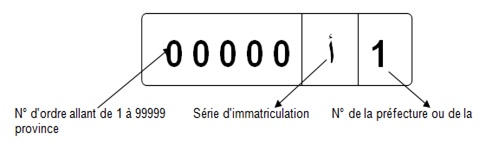
\includegraphics[width=\textwidth]{plaqueVehiculeAutomobile}
                \caption{Modèle sur 1 ligne pour les véhicules automobiles}
            \end{subfigure}
            \hfill
            \begin{subfigure}{0.3\textwidth}
                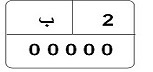
\includegraphics[width=\textwidth]{plaqueVehiculeAutomobileArriere}
                \caption{Modèle sur 2 lignes pour les véhicules automobiles}
            \end{subfigure}
            \hfill
            \begin{subfigure}{0.3\textwidth}
                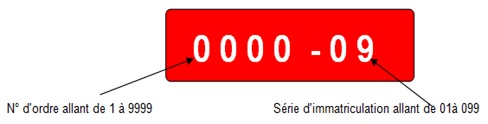
\includegraphics[width=\textwidth]{plaqueRemorqueSup750}
                \caption{Modèle pour les remorques d'un PTAC > 750 Kg}
            \end{subfigure}

            \begin{subfigure}{0.3\textwidth}
                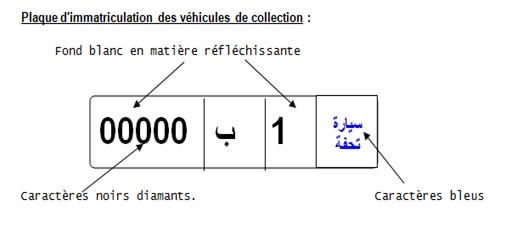
\includegraphics[width=\textwidth]{plaqueVoitureCollection}
                \caption{Modèle pour les véhicules de collection}
            \end{subfigure}
            \hfill
            \begin{subfigure}{0.3\textwidth}
                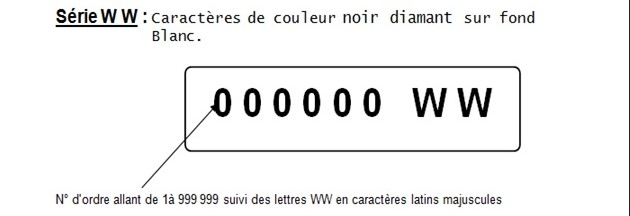
\includegraphics[width=\textwidth]{plaqueSerieWW}
                \caption{Modèle dans la série spéciale WW}
            \end{subfigure}
            \hfill
            \begin{subfigure}{0.3\textwidth}
                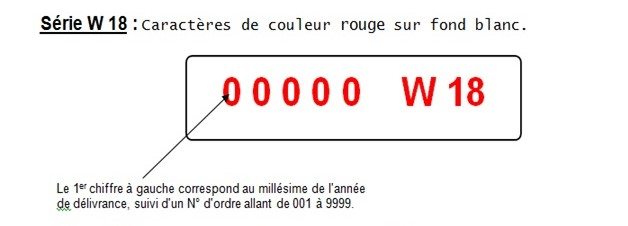
\includegraphics[width=\textwidth]{plaqueSerieW18}
                \caption{Modèle dans la série spéciale W18}
            \end{subfigure}

            \begin{subfigure}{0.3\textwidth}
                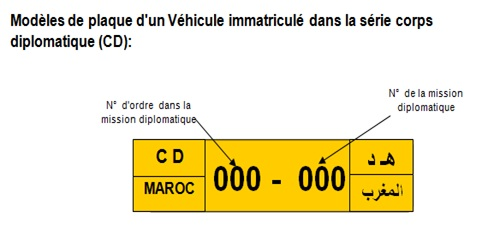
\includegraphics[width=\textwidth]{plaqueVehiculeCorpsDiplomatique}
                \caption{Modèle pour les véhicules de corps diplomatique}
            \end{subfigure}
            \hfill
            \begin{subfigure}{0.3\textwidth}
                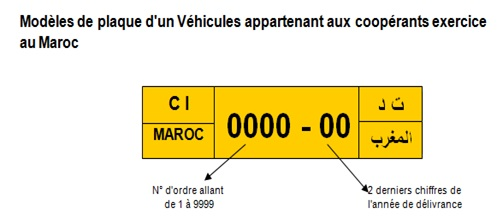
\includegraphics[width=\textwidth]{plaqueVehiculeCooperants}
                \caption{Modèle pour les véhicules des coopérants}
            \end{subfigure}
            \hfill
            \begin{subfigure}{0.3\textwidth}
                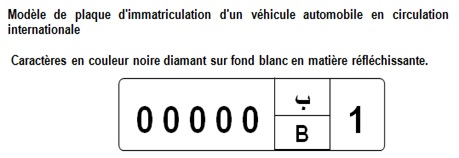
\includegraphics[width=\textwidth]{plaqueVehiculeACirculationInternationale}
                \caption{Modèle pour les véhicules en circulation internationale}
            \end{subfigure}
            \caption{Modèles de plaques d'immatriculation marocaines}
        \end{figure}
    En considérant ces caractéristiques, notre système doit prendre en entrée des images ou vidéos de véhicules au Maroc et être capable d'extraire l'ensemble des  numéros de plaques s'y trouvant pour un enregistrement dans une base de données.

    \subsection{Problèmatique et Objectifs du projet}
    Le projet surlequel nous avons travaillé est la résultante de deux constats majeurs faits sur le trafic routier au Maroc:
    \begin{enumerate}
            \item Le premier est lié à l’\textbf{augmentation rapide du nombre de véhicules en circulation dans le Royaume chérifien}.  Cette croissance accroît l’ampleur des problèmes liés au trafic routier comme le vol des voitures, les congestions, la violation des codes routiers et bien d’autres encore. 
            \item Le second  est lié au \textbf{système actuel de gestion de parking dit intelligent} et particulièrement la méthode actuelle pour ouvrir la barrière afin d'accéder à la zone de stationnement. Pour le moment, la plupart des systèmes implémentés dans le pays utilisent régulièrement des cartes \acrshort{rfid}. Ce qui rend le système pas vraiment automatisé de bout en bout.
        \end{enumerate}
    Face à ces constats, l’entreprise KF2Y Consulting dans sa démarche de création des villes intelligentes destinées au marché marocain a voulu mettre en place un système automatique de bout en bout pour la reconnaissance des plaques d’immatriculation marocaines.  Cette mission nous a donc été confiée dans le cadre de notre projet de fin d'études avec les objectifs suivant:
        \begin{enumerate}
            \item \textbf{Mettre en place un système \acrshort{anpr} spécifique aux plaques marocaines appelé \textit{MoPlaZer} performant (rapide et précis)}: Ce système doit être en mesure de localiser d’une part  les plaques d’immatriculation sur une image ou une vidéo et d’autre part extraire sous format alphanumérique leur numéro d’immatriculation.
            \item \textbf{Concevoir et développer une application mobile qui intègre le système}: L’application doit proposer deux modes de traitement
                \begin{itemize}
                    \item \textbf{Un mode statique}: Ici le système \acrshort{moplazer} traite les images fixes prises par une capture ou récupérées dans l’appareil mobile.
                    \item \textbf{Un mode temps réel}: Ici le système traite les séquences d’images continues (mode vidéo) à travers la caméra de l’appareil mobile
                \end{itemize}
            \item \textbf{Intégrer le système \acrshort{moplazer} dans un système embarqué pour un smart parking}: En effet le système \acrshort{moplazer} devra fournir sous format texte le numéro des plaques d’immatriculation des véhicules qui viennent à l’entrée du parking. Par la suite une vérification de l’existence du matricule détecté dans une base de données est faite. Dans le cas où le matricule se trouve dans la base de données, on déclenche l’ouverture de la barrière qui donne accès aux zones de stationnement.
        \end{enumerate}


